\documentclass{llncs}
\usepackage[colorlinks,allcolors=blue]{hyperref}
\usepackage[T1]{fontenc}
\usepackage{listings}
\usepackage{graphicx}
\usepackage{amsfonts}
\usepackage{verbatim}
\usepackage{cite}
\usepackage{booktabs}
\usepackage{multirow}



\graphicspath{{./images/}}

\begin{document}

    \title{Quality assurance of digital twins -- An experience report in the automotive industry}

    \author{Georg Hackenberg\inst{1}
    \and
    Alican Tüzün\inst{1}
    }
    \institute{School of Engineering\\
    University of Applied Sciences Upper Austria\\
    4600 Wels, Upper Austria, Austria\\
    \email{lncs@springer.com}}
    
    \maketitle

    \begin{abstract}
        Digital twins are becoming more and more important for the efficient and effective development and operation of cyber-physical systems.
        However, digital twins are only useful if they reflect the real-world system accurately enough, i.e.\ their quality is high enough.
        This claim entails the question, of what the term quality in the context of digital twins means and how it can be measured.
        In this article, we present our experience with the quality assurance of a digital twin for an assembly line in the automotive industry.
        We explain our preliminary definition of digital twin quality, which we derive from classical quality models for general software systems.
        Furthermore, we describe quality issues, which we were able to detect in a digital twin of an assembly line in the automotive industry.
        Finally, we conclude how to leverage our experience in different contexts and how to generalize the underlying approaches.
    \end{abstract}

    \section{Introduction}\label{section:introduction}
    
    The notion of the digital twin, which has gained popularity in 
    recent years, is often subject to vague and ambiguous envisions\cite{Review1}.
    The mispresenting of this notion began with the physical twin of the Apollo 13 spacecraft. 
    The twin of Apollo 13 was merely a tangible replication of the spacecraft that has been utilized in physical simulations. 
    Even though the digital aspect was expected to be present, there wasn't\cite{GrievesApollo13}.
    Another physical twin is the historic D-day map (also known as the Big Board) in Southwick House England, 
    which was used simultaneously before and during the operation, and can be argued to be similar. 
    The board was a twin of the operation, and it included models of battalions and ships that reflected the actual 
    locations of the corresponding formations. Furthermore, synchronization was 
    implemented to give directives from the real system to control the operation 
    flow and to update the physical twin state\cite{AMRC}.
    In contrast, a digital twin is a virtual counterpart of a real system, which should 
    be synchronized with a selected frequency and fidelity\cite{Review1,Review2,digitaltwinconsortium2022}.
    
    The envision of a digital twin emerged from Grieves'es conceptual model, which was called mirrored spaces model in 2002~\cite{Originsofdigitaltwinconcept},
    and later referenced in a 2005 journal article~\cite{2005JournayArticle}. 
    Furthermore, he introduced the information mirroring model, which was his ideal product lifecycle management tool with only one goal. 
    The goal was to gather as much information about the real system to minimize the waste of the system's sources such as energy, 
    time and material. Initially, this model had four main parts of a real system, 
    virtual system, connection between the real and virtual system and virtual simulations\cite{GrievesPLMBook}. 
    Later, Grieves removed the latter, to simplify the model\cite{Originsofdigitaltwinconcept}. Furthermore, after co-authoring with Vicker in 2010, 
    Grieves decided to use the NASA-invented Digital Twin word, instead of the information mirroring model\cite{Originsofdigitaltwinconcept}.
        
    Digital twins are highly intricate and adaptable systems that possess the capability to not only respond to environmental 
    changes but also modify their internal structure \cite{ZHANGUPDATEMETHOD, MobusSystemTheory}. Therefore, ascertaining a 
    requisite level of quality for the construction of a digital twin is an arduous undertaking.

    FELICE is a complex system that addresses a critical problem in robotics which is the effective integration of human and robot abilities in a collaborative setting. 
    This challenge requires the development of sophisticated algorithms and techniques that facilitate seamless communication, cooperation, and coordination between humans and robotic agents. 
    By addressing this issue, FELICE tries to represent a significant advancement in the field of robotics and has the potential to enhance the effectiveness and efficiency of a wide range of 
    human-robot collaborative tasks with the consideration of safety~\cite{FELICE}.

    The main purpose of this study is to inspect several artifacts and map the found issues to quality attributes to evaluate the quality of the digital twin for the FELICE project, which is currently in the design phase.~\cite{FELICE}. These artifacts included process videos showing the current 
    assembly procedure, a scope definition, a requirements specification, a general and operational conceptual model, 
    and a discrete event simulation module. We assessed the quality of these artifacts based on five crucial quality attributes: correctness, completeness, fidelity, efficiency, and evolvability.

    %%
    %%\subsection{Research objective}
    %%Find an approach to assess the quality of Digital twins~\cite{Jones2020}

    %%\subsection{Research question}\label{section: Research Questions}
    %%What is the quality of digital twins?
    %%What is the state art of digital twin quality?

    %%\subsection{Research methodology}
    %%TODO

    \section{State of the art on quality}
    Oxford English Dictionary describes the word quality either as a noun or an adjective. 
    The adjective form indicates, a high standard or excellence. For example, the phrase quality products imply 
    that quality adds a high standard state to the product. Several definitions describe quality 
    as a noun, however, the impactful definition is the quality as a standard of an entity which is measured against the 
    different or the similar entities\cite{OxfordDictionary}. This definition clearly shows the relativity of quality. In addition, quality is defined 
    as the degree to which a set of inherent properties of an entity fulfills the given requirements~\cite{ISO9000}.    
    \subsection{Product quality and Management}
    A product is a tangible or intangible system that satisfies the needs or wants of a customer. It could be a physical system like a car, or an abstract system, like a digital twin. 
    Regarding product quality, there are two different aspects~\cite{GrievesPLMBook}.
    First, quality is an attribute of a product, which meets product specifications. Specifications are mostly defined by the supra-systems subsystems, 
    such as by the stakeholders within the supra-system,  If the stakeholders' expectations, or needs, are met, we can consider high quality.
    The ability to execute to a specific usage standard is the second facet of product quality. Since this standardization is usually not controllable, 
    unlike the first, the system's quality will be determined by how the implied or obligatory standards are fulfilled.


    Quality management systems(QMS) function to plan and execute the organization's quality policies and goals. 
    Examples of such systems can be a standard like ISO 9001 which can provide a framework for an organization, or a data-driven methodology such as Six Sigma to reduce defects and improve efficiency. 
    These concepts are not new, for example, ISO 9001 standard has been established in 1987, and is still being regularly updated ~\cite{ISO90012015}. 
    \subsection{Software quality}
    Software is a combination of programs and data which can be used by virtual 
    systems as well as a physical system like a computer system. In contrast, hardware 
    is a physical subsystem of a computer system\cite{OxfordDictionary}. 

    Software Quality is determined by how well software fulfills the requirements that were set. However, those requirements  
    not always reflect what the stakeholders need, hence the quality depends on how accurately these requirements were set \cite{IEE730-2014}. 
    As a result, functional suitability, performance efficiency, compatibility, usability, reliability, security, maintainability 
    and portability is the standardized eight attributes that measure software quality \cite{ISO/IEC:25010}.
    
    Software quality management techniques come from already used manufacturing techniques in the industries. For example, product quality assurance has been used as a 
    software quality management activity with some modifications. For example, in manufacturing, products will never exactly meet a specification, due to errors in the machining which results in some tolerance area. 
    But in the software systems, or more precisely in the virtual systems, it's most of the time, not the case. Also, it's nearly impossible to conclude that, 
    the software product fully meets its specifications. 
    Hence, most of the quality assessments are subjective processes and as a result, the quality attributes should be inspected subjectively \cite{SoftwareEngineering}.  

    \subsection{Simulation Quality}
    Simulation models are not merely virtual systems; they are also abstracted systems, 
    which are nothing more than imitations or, to be more precise, abstractions of real systems. 
    Every day, simulation of the real systems occurs in the human brain when the prediction of the future outcome or about the 
    past state of some occurred event required\cite{MobusSystemTheory}. However, most of the simulation processes are computer-based with software programs. Consequently, the idea of simulation software programs emerges. 
    For example, ANSYS\cite{Ansys}, ABAQUS\cite{Abaqus}, and AnyLogic\cite{AnyLogic} are examples of these simulation software programs. 

    Validation and verification are used to evaluate the quality characteristics of the simulation 
    model \cite{StewartSimulation,VerificationValidationSergent,OsmanBalci}. 
    Validation is the process of evaluating the simulation quality of the model in comparison to 
    the real system from the perspective of the model's intended applications.
    On the other hand, verification is a procedure to 
    evaluate a simulation model's implementation and its associated 
    data concerning the conceptual description and specifications of the 
    model developer\cite{StewartSimulation,VerificationValidationSergent}.

    Various validation and verification techniques can be employed, which can be broadly categorized into six areas: informal, static, dynamic, symbolic, constraint, 
    and formal techniques \cite{balcicategories}\cite{balcitechniques}. Formal techniques involve mathematical formality, whereas informal techniques rely on human intervention 
    and reasoning. Although mathematical techniques are more precise, informal techniques 
    are more commonly used \cite{balcicategories}. Also, the use of informal techniques does not imply a lack of structure, but rather a reliance on human expertise and interpretation \cite{balcitechniques}.
    \subsection{Digital twin quality}
    To analyze the state of the digital twin quality, a literature analysis was executed. 
    The analysis especially focused on how the digital twin quality is mentioned and assessed within the academic dissertations.

    \subsubsection*{Literature Search Methodology}
    To conduct a thorough literature review on digital twin publications, tools such as Google Scholar and Scopus are utilized. Due to the vast amount of available literature, it is necessary to narrow down the scope of the research. 
    Therefore, a multi-level filtering algorithm is employed to refine the search results.

    The first level of filtering for the literature review on digital twin publications involves specific criteria. These include that dissertation must be written in English and 
    published in a journal or conference and that the search term must be an exact match. To execute this initial filtration, 
    the following queries are used for Google Scholar and Scopus respectively: "search term" and ALL ("digital twin quality") AND (LIMIT-TO (LANGUAGE, "English")).

    After the initial filtering, a second level of manual investigation is necessary. The following criteria are used for this level of filtering:    
    \begin{itemize}
        \item  Eliminating duplicates
        \item  Removing dissertations that are not in English
        \item  Ensuring that selected dissertations have a proper literature review
        \item  Ensuring that abstract and conclusion are relevant to the search term
    \end{itemize}
    If an interesting dissertation(s) would be found during the reading, it will be checked again with the initial filter.
    \subsubsection*{Literature Search Result}
    The search for "digital twin quality" initially resulted in 41 hits on Google Scholar and 3 on Scopus. 
    After the second level of filtering, 6 duplicate dissertations were removed and 10 dissertations that were not in English were also eliminated. 
    This left only 9 dissertations that met all the criteria and were reviewed.

    The search for "digital twin verification" initially resulted in 19 hits on Google Scholar and none on Scopus. 
    After the second level of filtering, one duplicate dissertation was removed and two dissertations that were not in 
    English was also eliminated. As a result, all dissertations were rejected.

    The search for "digital twin validation" initially resulted in 59 hits on Google Scholar and none on Scopus. 
    After the second level of filtering, 4 duplicate dissertations were removed and 4 
    dissertations that were not in English were also eliminated. This left only 8 dissertations that met all the criteria and were reviewed.
    
    After a thorough review of 17 research papers, several significant findings were revealed.
    
    First, it was noted that Shcherba et al. focuses on the importance of model quality as an observation for a digital twin subsystem. 
    However, they acknowledged that the quality assessment of the digital twin cannot solely rely on models~\cite{Shcherba}. 

    He Zhang et al. developed a consistency evaluation approach for digital twin models, which can be used to assess their quality. 
    The authors also discuss essential concepts, such as consistency between real and virtual systems and ultra-fidelity models. 
    This article emphasizes the improvement of the service component of the digital twin~\cite{ZHANGEVALUATIONMETHOD}.

    He Zhang et al. introduced the updating method for digital twin models in yet another insightful article.
    Once more, the accuracy and coherence of the model concepts were addressed~\cite{ZHANGUPDATEMETHOD}.

    Selch et al. present a machine-learning approach based on Bayesian networks to track the quality of the digital twin. 
    The unique aspect of this study is that the authors determine the contributions of subsystems to forecast the overall quality of the digital twin, 
    rather than just analyzing it as a single system. The digital couplings, which are linkages between the subsystems, are also identified as a source of extra uncertainty. 
    However, since only one digital twin has been used in practice, multiple subsystem digital twins have not been validated~\cite{QualityMonitoringofCoupledDigitalTwins}.

    Additionally, the stability of digital twin models was assessed by another study using the Kolmogorov-Smirnov statistical test, 
    which measures the degree of similarity between the probability distribution of the model's predictions and the distribution of the actual data~\cite{RadarDigitalTwin}.

    Edward Y. Hua et al. identify five open problems with digital twin model validation, including modeling realism, data uncertainty, system dynamics, use-case alignment, and reporting invalid modes. To address these challenges, the authors propose a digital-twin model validation framework. The paper also highlights three areas for future research, 
    including uncertainty and sensitivity analysis, model validation of system-of-systems, and combining expert knowledge and collected data ~\cite{ValidationofDigitalTwins}. 

    Finally, Shotaro Hamato et al. demonstrated successful real-time anomaly detection using the Unscented Kalman Filter with the digital twin model. 
    However, determining the appropriate threshold for anomaly detection remains an issue~\cite{JapeneseKalmanFilterCorrectness}.

    Overall, these studies provide valuable insights into various aspects of digital twin quality assessment, 
    including model consistency, stability, and validation, as well as machine learning-based approaches and real-time anomaly detection. 
    However, the identified open problems, including modeling realism, data uncertainty, system dynamics, use-case alignment, and reporting invalid modes, 
    call for further research in the field to improve the quality and reliability of digital twins. Moreover, 
    the lack of well-defined quality parameters for digital twins poses a significant challenge in ensuring their quality,
    which necessitates the development of appropriate quality metrics and standards for digital twins.
    \subsection{Digital Twin Quality Attributes}\label{section:Digital Twin Quality Attributes}
    We consolidated our findings from various standards, including ISO/IEC:25010, IEE730-2014, ISO9000, and ISO9001, as well as consulted the  Oxford dictionary to 
    synthesize our findings\cite{ISO9000,ISO90012015,ISO/IEC:25010,IEE730-2014, OxfordDictionary}.
    
    \textbf{Correctness} is a  derived word from the adjective correct, which means that something is error-free regarding fact or truth. In the context of the digital twins, our fact or truth is a real system hence, correctness is a grade of quality, that indicates an error between the real system and a digital twin system.
    Meanwhile, the quality of being correct is described by the term accuracy \cite{OxfordDictionary}. 
    
    \textbf{Completeness} is a derived word from the word complete, which can be described as an adjective, attribute, or verb\cite{OxfordDictionary}. 
    The adjectival form of complete is a state of having all the necessary or appropriate parts\cite{OxfordDictionary}.

    \textbf{Fidelity} refers to the degree of exactness with which the real system is copied and represented. Low fidelity indicates a simplified representation, 
    while high-fidelity refers to an accurate and detailed representation of the real system \cite{Review2}. 
    The concept of fidelity has garnered significant attention in recent years and continues to be an important area of research in digital twins\cite{Review2}\cite{Review1}.

    \textbf{Efficiency} refers to the quality of being efficient, and efficiency is achieving
    maximum productivity with minimum wasted effort or expense. The concept of efficiency is tightly coupled to productivity, which refers to the quality of being productive,
    also the word productive can be explained as producing or being able to produce large amounts of goods\cite{OxfordDictionary}.  
    For example, time efficiency indicates that,  with less amount of time as an input, more output with the minimum 
    waste during the process is desired. Goods of the digital twin are nothing but information, which Grieves first 
    indicated with this Information Mirror Model\cite{GrievesPLMBook}.

    \textbf{Evolvability} is a system's capability to enhance its suitability to its environment through alterations to both its internal and functional 
    structure\cite{MobusSystemTheory}. Another term to describe the response to changes in the environment is adaptability.
    However, this concept differs from evolvability in that it only affects a system's internal or functional structure temporarily. 
    For instance, a digital twin, which is a virtual system, can be designed to be more flexible and scalable, 
    allowing for easy updates and the addition of new features. 
    These updates and new features will result in definite changes to the structure of the system. 
    On the other hand, a responsive web design is an adaptable system, capable of adjusting its size and layout 
    depending on the user's hardware. As we have seen in \cite{ZHANGUPDATEMETHOD}, the update method shows that digital twins are evolvable systems, 
    hence this attribute should be considered when the digital twin's quality is inspected. To assess the evolvability attribute, scalability analysis,
    reusability analysis, modifiability analysis, testability analysis, and maintainability analysis can be performed. 
    %%%%%%%%%%%%%%%%%%%%%%%%%%%%%%%%%%%%%%%METHODS%%%%%%%%%%%%%%%%%%%%%%%%%%%%%%%%%%%%%%%
    \section{Artifacts and Methods}
    The used methodology consists of manual artifact reviews and evaluation of the results according to the digital twin quality attributes.    
    \subsection{Artifacts}\label{section:Artifacts}
    The current stage of review encompasses five key artifacts, including process videos displaying the current assembly procedure without an adaptive workstation and cobot, a scope definition outlining the objects on the shop floor requiring tracking or twinning, a requirements specification summarizing functional and non-functional requirements for the digital twin, a general and an operational conceptual model elucidating the high-level structure of the assembly procedure, 
    and a discrete event simulation module that implements the structures prescribed by the conceptual models.

    \textbf{Process Videos:}
    The project partner provided three videos initially to explain the manual assembly procedures performed at each of the three workstations. From the videos,  
    the sequence of assembly steps was extracted at least for one product variant. The tools and the parts needed for each assembly operation were observed. Additionally, the approximate duration of each assembly step 
    was estimated, and some ergonomic characteristics of each operation were derived. 
    The derivable ergonomic characteristics mainly included the poses and motions performed by the operators.

    \textbf{Scope Definition:}
    To better understand the context and focus of the digital twin, 
    the project partner used a methodology based on hierarchical task analysis and the process videos. 
    This resulted in a scope definition that identified entities to be twinned, entities to be tracked, and important areas in the scene. 
    Entities to be twinned needed to be represented accurately in the simulation models, including their position, pose, speed, fatigue, and other state variables. 
    Entities to be tracked, on the other hand, only required position information. The scope definition was based on a floor plan of the production facility, with the three workstations marked as gray rectangles. 
    The human workers, cobot, and adaptive workstation were identified as entities to be twinned, and therefore required accurate representation, 
    monitoring, and simulation. Other entities, such as an AGV, carts with doors, and screwdrivers used for assembly operations, were designated as entities to be tracked.

    \textbf{Requirements Specification} for the digital twin was defined with a unique ID, a natural language description, an origin, a category, a priority, and a rationale. The ID was used as a reference point for other project artifacts, while the specification described the requirement in a way that allowed for testing of the digital twin implementation. The origin of the requirement was noted to identify the project partner responsible for its creation. The category distinguished between functional and non-functional requirements, as well as constraints and standards. The priority of each requirement was classified into four levels 
    (must-, should-, could-, and would-have) to help prioritize development efforts. 
    Finally, the rationale provided a clear explanation for each requirement's inclusion in the specification.

    \textbf{Conceptual Model} was comprised of two parts:  a general conceptual model and an operational conceptual model. Both models described the assembly line processes, but the operational conceptual model focused on the specific steps of the assembly process, while the general conceptual model focused on higher-level processes and workflows.
    The general conceptual model was represented using a general flow chart notation that distinguished between a root node, activity nodes, and decision nodes.
    The operational conceptual model consisted of three spreadsheets, each displaying the sequence of assembly operations performed at one workstation. 
    The assembly operations were divided into macro- and micro-operations, with each macro-operation referring 
    to one part of the final product being assembled, and the micro-operations referring to the individual steps needed to complete the respective macro-operation.

    \textbf{Discrete Event Simulation Model} consisted of seven sections, including two animation sections, two input sections, one output section, one process logic section, and a database section. The animation sections provided a two-dimensional and a three-dimensional representation of the system, which aided in understanding the simulation and for debugging purposes. The input sections allowed for the management of inputs to the simulation model, and the output section displayed summary performance indicators about the simulation run. 
    The process logic section contained the process building blocks, such as queues and assembly operations. The database section provided an interface to data sources and sinks.
    
    \subsection{Manual Artifact Reviews and Evoluation}
    During the initial stages of the project, when the target system was not yet available, there was a lack of observable data about system behavior that could be utilized for validation. 
    Instead, informal and potentially incomplete, inconsistent, or incorrect system descriptions had to be relied upon. Therefore, manual reviews were deemed the most suitable tool to account for the characteristics of this situation.
    The manual review included, audits, inspections, reviews, structural analysis 
    and walkthroughs with the project partners which was inspired by Balci's manual review works \cite{balcitechniques}. Lastly, observations after the reviews were mapped to the quality attributes. 
    %%%%%%%%%%%%%%%%%%%%%%%%%%%%%%%%%%%%%%%RESULTS%%%%%%%%%%%%%%%%%%%%%%%%%%%%%%%%%%%%%%%
    \section{Results}
    %%TODO WRITE HERE ONCE AGAIN
    

    \begin{table}[h!]
        \begin{center}
          \caption{Mapping findings to Quality Attributes: Results of the manual artifact reviews were mapped to quality attributes, which were discussed in \ref{section:Digital Twin Quality Attributes}}
          \label{tab:Mapping}
          \begin{tabular}{l@{\hspace{1cm}}l} 
            \textbf{Findings} & \textbf{Missing Quality Attribute}\\
            \hline
            Findings 1, 2 and 6 &     Completeness\\
            Findings 3, 12, 14,15 and 17  &     Correctness, Completeness\\
            Findings 4 &     Correctness\\
            Findings 5,9,11,16,20 and 21 &     Evolvability\\
            Findings 7 &     Correctness, Completeness, Fidelity, Efficiency, Evolvability\\
            Findings 8 &     Completeness, Fidelity, Evolvability\\
            Findings 10 &    Correctness, Completeness, Fidelity, Evolvability\\
            Findings 13 and 19 &    Completeness, Evolvability\\
            Findings 18&Correctness, Efficiency \\
    \end{tabular}
    \end{center}
    \end{table}



    \begin{figure}[htbp]
        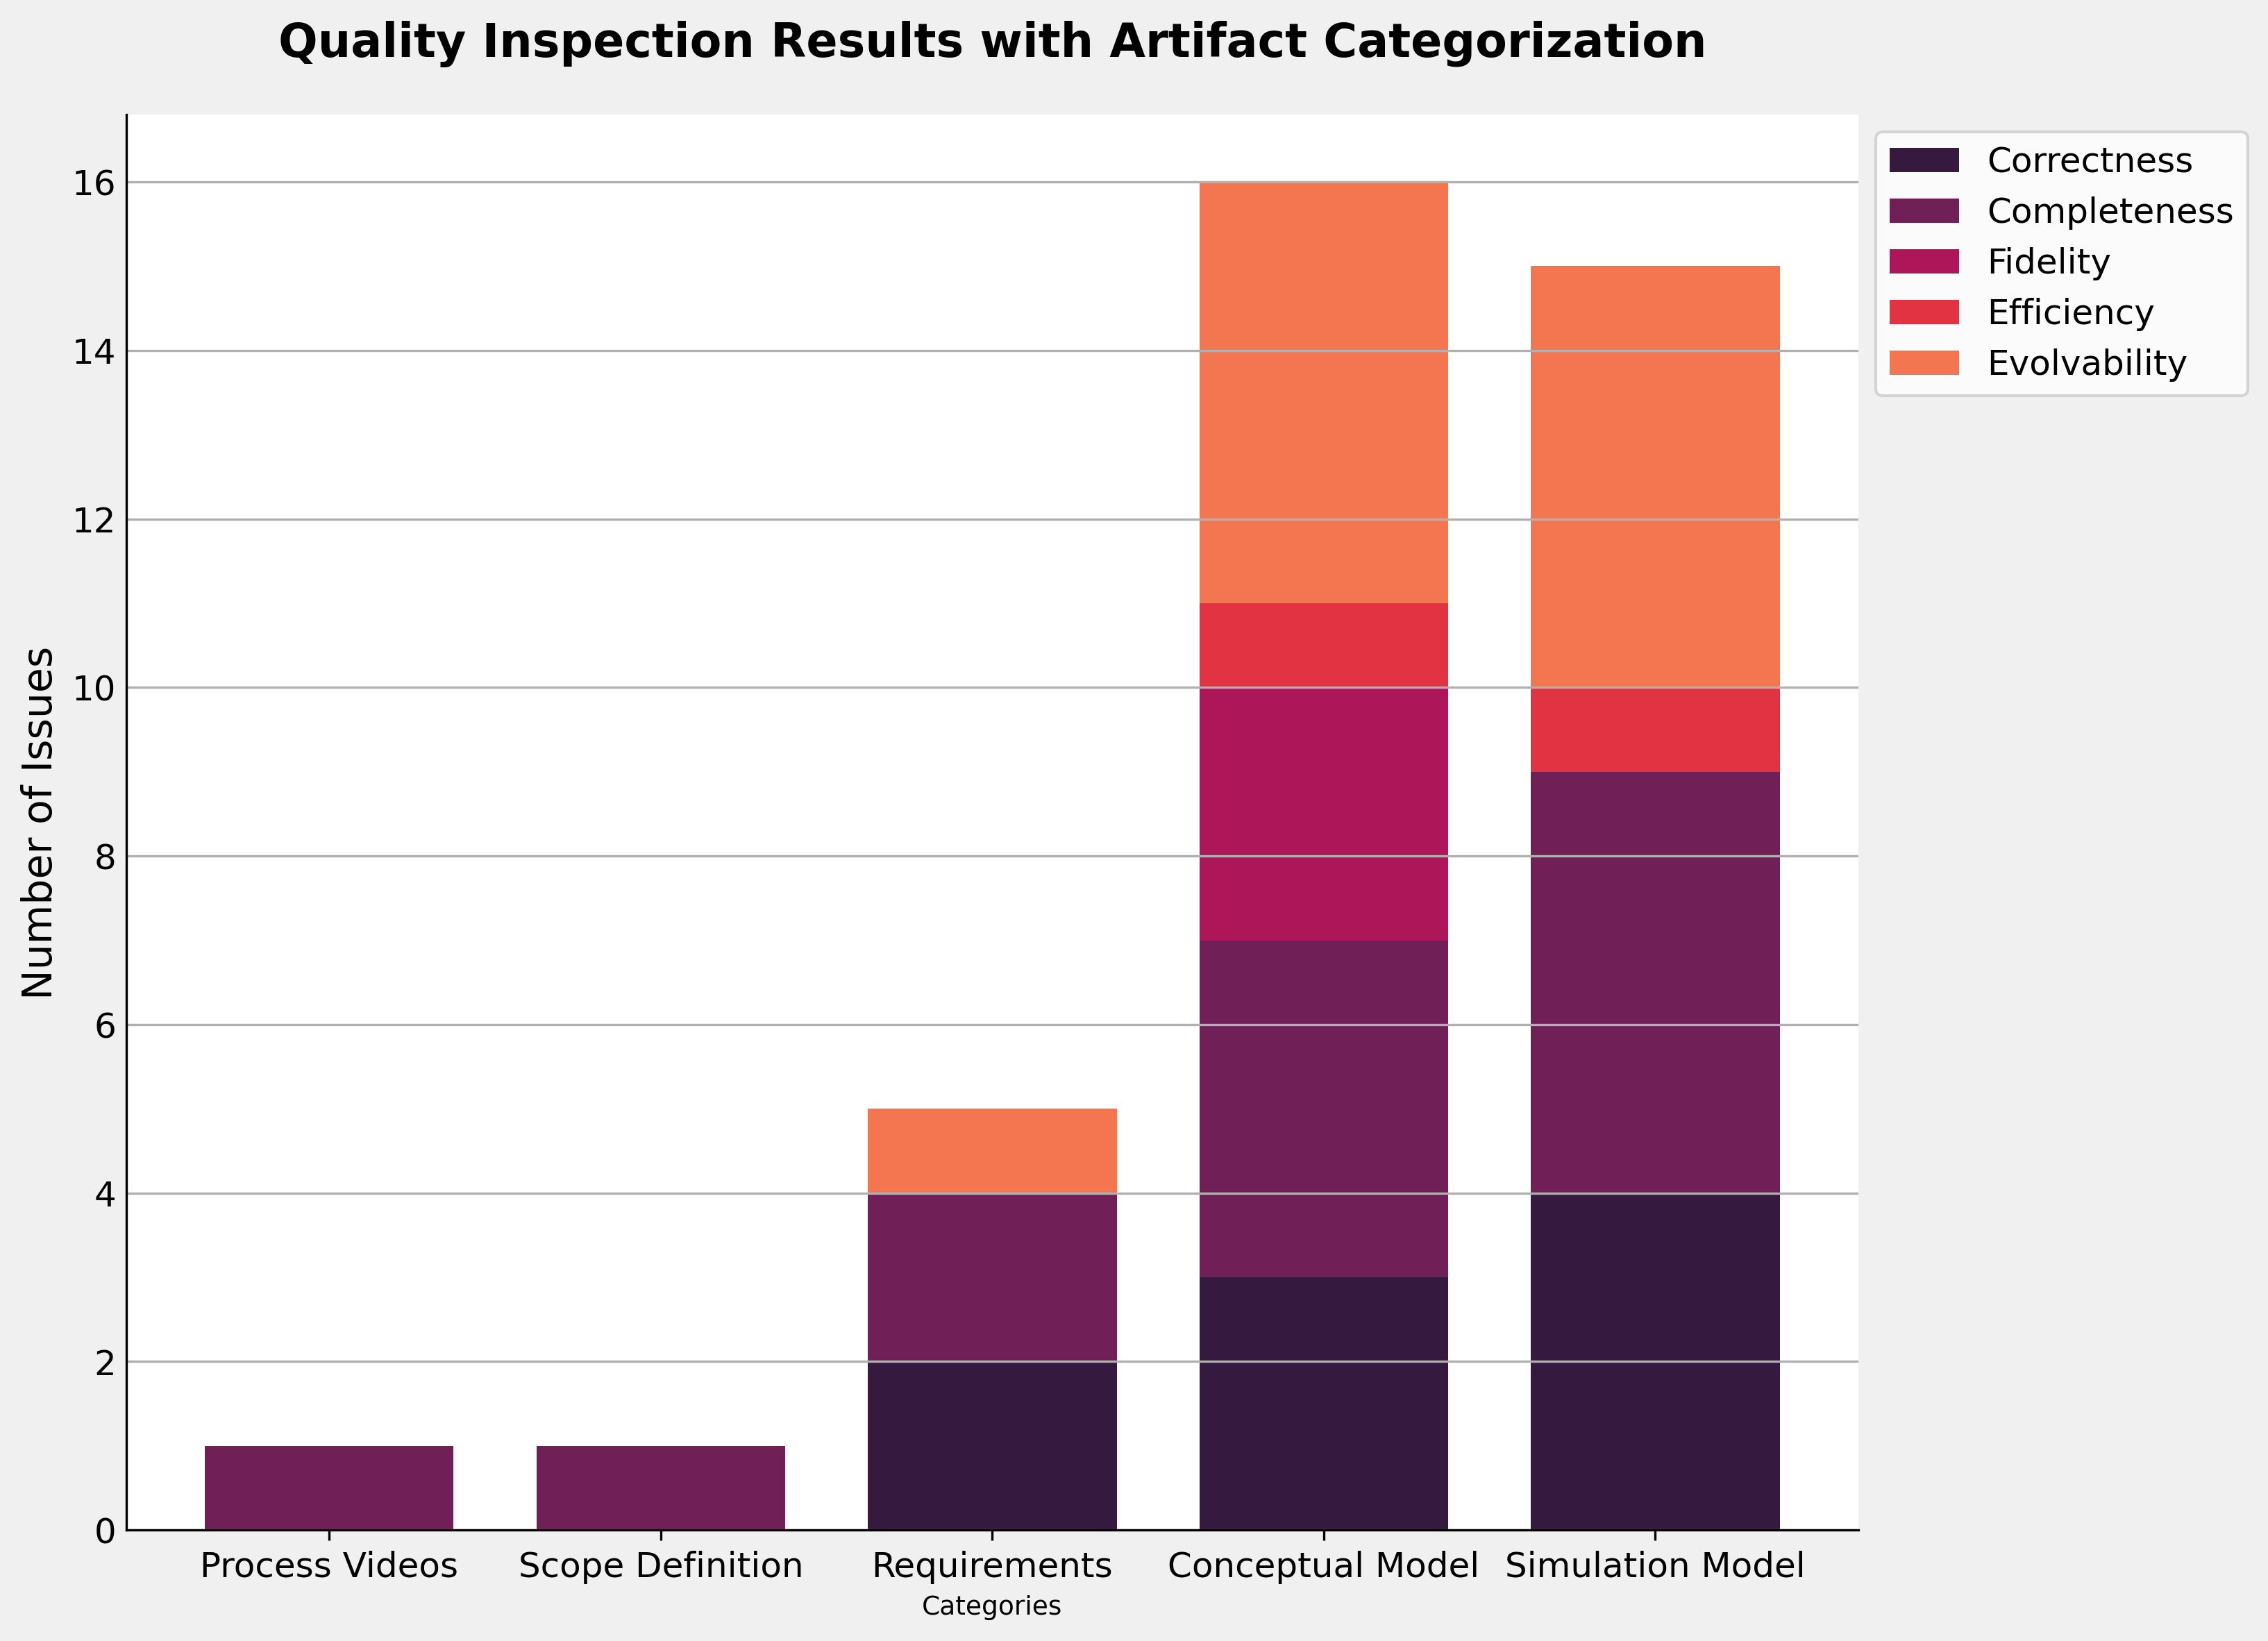
\includegraphics[scale = 0.40]{quality_inspection_results_with_artifacts.png}
        \caption{Quality Inspection Results Categorized with Artifacts: X-Axis represents artifacts in \ref{section:Artifacts}, Y-Axis represents the number of missing quality attributes found for each artifact, 
        and lastly, each digital twin quality attribute is shown by the colors.}
        \label{fig:QualityInspectonResultsWithArtifacts}
    \end{figure}

    \textbf{Process Videos Review Results}

    Findings 1  - Even though the videos are well suited for providing a first impression of the production facility 
    and the current assembly process for one product variant, the other product variants include different assembly operations, 
    which were not shown in the videos. 
    Furthermore, the cobot and the adaptive workstation were not part of the assembly process yet,
     hence the videos do not provide a complete representation of the target system.  

    \textbf{Scope Definition Review Results}

    Findings 2 - The scope definition focuses on the physical entities of the shop floor and is consistent with the videos presented in the previous section. 
    However, the scope definition is incomplete. Several entities are only selected for the tracking, hence additional state information such as the failure status of these entities was missing in the digital twin. 

    \textbf{Requirements Specification Review Results}

    Findings 3 - Atypical categorization of the digital twin requirements as functional, non-functional, constraint and standard was introduced. 
    Also, standard categories were considered as a cause of requirements instead of a category of requirements. Furthermore, 
    the constraint category was considered a non-functional requirement which results in a significant misunderstanding between non-functional 
    requirements and constraints. Finally, some requirements were described as non-functional requirements instead of functional requirements. 

    Findings 4 - Imprecise and unclear statements were found in requirement specifications. 

    Findings 5 - Key design decisions were found in the requirement specifications, which results in a considerable decrease in maintainability. 

    \textbf{Conceptual  Model Review Results}

    Findings 6 - Conceptual models are not designed to react to unwanted situations. 

    Findings 7 - Conceptual model specification was not clear enough, which results in quite some room for interpretations by the stakeholders. 
    as the use of an unspecified flow chart model is prone to differing interpretations by different stakeholders and probable incorrect understanding of the relations between the sub-systems.

    Findings 8 - The difference between the event triggers and decision nodes was not clear, which decreased the clarity and maintainability of the model considerably. 

    Findings 9 - The representation of the model is not great, hence understanding the interactions between the different subprocesses are not clear.

    Findings 10 - The model were lacking great organization tools such as swim lanes and object flows. 

    Findings 11 - The assignment of the cobot to micro-operations was not regularly reviewed and updated as the project progresses. 

    Findings 12 - Even though the durations of the macro-operations were well-known and studied thoroughly before, the durations of the micro-operations were estimated based on a simple calculation scheme.

    \textbf{Discrete Event Simulation Model Review Results}

    Findings 13 - The input controls in the simulation module was not complete or aligned with the actual inputs that will be provided by another system. 

    Findings 14, and 15 - The ranges defined for some events were not validated. 

    Findings 16 - Database structures were not updated automatically, instead done manually.

    Findings 17 - The duration of micro-, loading- and unloading-operations of the cobot were based on assumptions rather than actual measurements.

    Findings 18 - The simulation module does not support parallel execution of micro-operations. 

    Findings 19 - The interruption mechanism of the assembly line was not considered within the simulation module. 

    Findings 20 - The number of micro-operations was hard coded, consequently, the simulation module must be reprogrammed every time, when a new micro-operation is needed. 

    Findings 21 - Edge cases were not considered in the simulation module.  


    \subsection{Mapping the Issues to Quality Attributes}
    The analysis revealed that a total of thirty-eight digital twin quality attributes were lacking in these artifacts. \ref{fig:QualityInspectonResultsWithArtifacts}
    Therefore, to evaluate the quality of the FELICE digital twin, observations are mapped to one or more relevant quality attributes\ref{tab:Mapping}.
    In addition, the assessment shows that every one of the identified issues was quickly attributed to a specific quality attribute.  
    Specifically, 24\% of the issues were related to correctness, which indicates an error between the real system and a digital twin system.
    35\% of the issues were related to completeness, proving that some necessary or appropriate parts are missing.
    8\% of the issues were related to fidelity, indicating a lack of detail. 5\% of the issues were related to efficiency, indicating poor 
    performance or excessive resource usage. Finally, 28\% of the issues were related to evolvability, indicating that the system has flexibility or scalability issues.  

    \section{Discussion}

    The results of this study demonstrate that a manual review and mapping of quality attributes to issues is an effective approach for evaluating the quality of digital twins in the design phase.  
    Therefore, systematic analysis of the identified issues in terms of their relevance to various quality attributes is an effective way to gain insight into the strengths and weaknesses of the digital twin system under development. 
    These insights can be used to guide further design decisions and improvements, ultimately leading to a higher-quality end product.

    The quality assessment of the digital twin encountered some limitations due to the exility of information about the real system. Some artifacts provided less information, such as process videos, which only provide a limited perspective of the shopfloor based on the camera's field of view and the skills of the video maker. 
    In contrast, the simulation and conceptual model offer a plethora of aspects to examine and assess, which results in a higher probability of discovering the issues \ref{fig:QualityInspectonResultsWithArtifacts}.



    
    \section*{Acknowledgements}
    TODO

    \bibliography{main}
    \bibliographystyle{splncs04}

\end{document}